% flashcards-title: The same four readings on two different vertical axes
% flashcards-desc: Two small graphs side by side labeled display P and display Q, each plotting four dots against days one through four. In display P the vertical axis is labeled from zero to fifty centimeters in steps of ten and the four dots sit at nearly the same height. In display Q the vertical axis is labeled from forty point zero to forty point five centimeters in steps of one tenth and the same four dots step visibly upward from left to right.
\documentclass[dvisvgm,tikz,border=8pt]{standalone}
\usepackage{tikz}
\usetikzlibrary{arrows.meta,calc,positioning}
\definecolor{DeckInk}{HTML}{172A3A}
\definecolor{DeckAccent}{HTML}{176B87}
\definecolor{DeckWarm}{HTML}{D97706}
\definecolor{DeckMuted}{HTML}{667784}
\definecolor{DeckPaper}{HTML}{F7FAFC}
\tikzset{
  every node/.style={font=\sffamily, text=DeckInk},
  object/.style={draw=DeckInk, line width=1.1pt, fill=DeckPaper},
  primary/.style={draw=DeckAccent, line width=1.5pt},
  boundary/.style={draw=DeckAccent, line width=1.5pt, dashed, rounded corners=6pt},
  guide/.style={draw=DeckMuted, line width=0.9pt, dashed},
  dimension/.style={{Stealth[length=3.2mm,width=2.2mm]}-{Stealth[length=3.2mm,width=2.2mm]}, draw=DeckWarm, line width=1.2pt},
  motion/.style={-{Stealth[length=3.5mm,width=2.5mm]}, draw=DeckAccent, line width=1.5pt, dashed},
}

\begin{document}
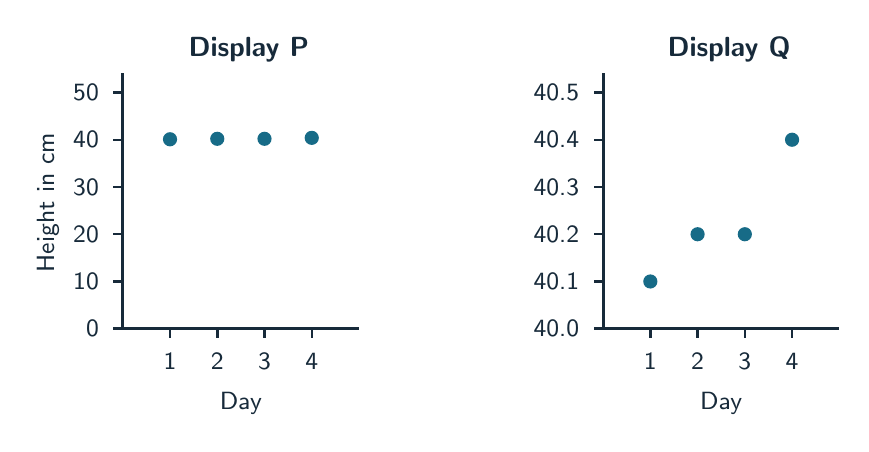
\begin{tikzpicture}[x=1cm,y=1cm]
  % Panel P: y = value * 0.06
  \node[font=\sffamily\bfseries] at (1.6,3.55) {Display P};
  \draw[DeckInk, line width=1.1pt] (0,0) -- (3.0,0);
  \draw[DeckInk, line width=1.1pt] (0,0) -- (0,3.25);
  \foreach \y/\v in {0/0,0.6/10,1.2/20,1.8/30,2.4/40,3.0/50}{
    \draw[DeckInk, line width=0.9pt] (0,\y) -- (-0.12,\y);
    \node[font=\sffamily\small, anchor=east] at (-0.18,\y) {\v};
  }
  \foreach \x/\v in {0.6/1,1.2/2,1.8/3,2.4/4}{
    \draw[DeckInk, line width=0.9pt] (\x,0) -- (\x,-0.12);
    \node[font=\sffamily\small] at (\x,-0.42) {\v};
  }
  \node[font=\sffamily\small] at (1.5,-0.95) {Day};
  \node[font=\sffamily\small, rotate=90] at (-0.95,1.6) {Height in cm};
  \fill[DeckAccent] (0.6,2.406) circle (0.09);
  \fill[DeckAccent] (1.2,2.412) circle (0.09);
  \fill[DeckAccent] (1.8,2.412) circle (0.09);
  \fill[DeckAccent] (2.4,2.424) circle (0.09);
  % Panel Q: y = (value - 40.0) * 6
  \begin{scope}[xshift=6.1cm]
    \node[font=\sffamily\bfseries] at (1.6,3.55) {Display Q};
    \draw[DeckInk, line width=1.1pt] (0,0) -- (3.0,0);
    \draw[DeckInk, line width=1.1pt] (0,0) -- (0,3.25);
    \foreach \y/\v in {0/40.0,0.6/40.1,1.2/40.2,1.8/40.3,2.4/40.4,3.0/40.5}{
      \draw[DeckInk, line width=0.9pt] (0,\y) -- (-0.12,\y);
      \node[font=\sffamily\small, anchor=east] at (-0.18,\y) {\v};
    }
    \foreach \x/\v in {0.6/1,1.2/2,1.8/3,2.4/4}{
      \draw[DeckInk, line width=0.9pt] (\x,0) -- (\x,-0.12);
      \node[font=\sffamily\small] at (\x,-0.42) {\v};
    }
    \node[font=\sffamily\small] at (1.5,-0.95) {Day};
    \fill[DeckAccent] (0.6,0.6) circle (0.09);
    \fill[DeckAccent] (1.2,1.2) circle (0.09);
    \fill[DeckAccent] (1.8,1.2) circle (0.09);
    \fill[DeckAccent] (2.4,2.4) circle (0.09);
  \end{scope}
\end{tikzpicture}
\end{document}
